\documentclass[11pt, oneside]{article} 	% use "amsart" instead of "article" for AMSLaTeX format
\usepackage{geometry} 		% See geometry.pdf to learn the layout options. There are lots.
\geometry{letterpaper} 		% ... or a4paper or a5paper or ... 
\usepackage[parfill]{parskip} 		% Activate to begin paragraphs with an empty line rather than an indent
\usepackage{graphicx}				% Use pdf, png, jpg, or eps� with pdflatex; use eps in DVI mode
								% TeX will automatically convert eps --> pdf in pdflatex		
\usepackage{amssymb}
\usepackage{amsmath}
\usepackage{amsthm}
\usepackage{authblk}
\usepackage{framed}
\usepackage[
backend=biber,
style=alphabetic,
]{biblatex}
\usepackage{graphicx}
\graphicspath{ {./images/} }
\usepackage{verbatim}
\usepackage{tikz} 
\usepackage{subcaption}
\captionsetup{compatibility=false}


\usepackage{tikz}
\usetikzlibrary{positioning, arrows.meta, decorations.pathreplacing}

\usepackage{syntonly}

% \syntaxonly \langle -- use this for checking syntax only
% \mbox {text} - keep together
% \fbox {text} - keep together and draw around

%\pagestyle{plain|headings|empty} % header and footer p.27
%SetFonts
%\include{filename}, \includeonly{filename1, filename2} , \input[fiename}

%SetFonts% 


\newtheorem{theorem}{Theorem}

\title{Proof of the Friendship Theorem}
\author{Dave Fetterman}
\date{\today}

\begin{document}

\maketitle

\begin{abstract}
A proof of the ``Friendship Theorem'', the problem proposed by Claude, solved by yours sincerely after many misstarts.

\end{abstract}


\begin{theorem}[The Friendship Theorem]
If everyone at a party has exactly one friend in common, then there is a person who is friends with everyone else.
\end{theorem}

\begin{proof}
Naturally, we model this as a graph.  Here is such a graph, where $v_2...v_5$ all share $v_1$ as a friend, and between $v_1$ and any other partygoer, one friend exists in common.

  \begin{figure}[h]
  \centering
  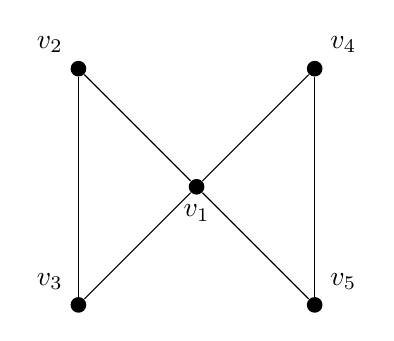
\begin{tikzpicture}[scale=1.5]
      % Vertices
      \node[circle, fill, inner sep=2pt, label=below:$v_1$] (v1) at (0,0)
  {};
      \node[circle, fill, inner sep=2pt, label=above left:$v_2$] (v2) at
  (-1,1) {};
      \node[circle, fill, inner sep=2pt, label=above left:$v_3$] (v3) at
  (-1,-1) {};
      \node[circle, fill, inner sep=2pt, label=above right:$v_4$] (v4) at
  (1,1) {};
      \node[circle, fill, inner sep=2pt, label=above right:$v_5$] (v5) at
  (1,-1) {};

      % Edges
      \draw (v1) -- (v2);
      \draw (v2) -- (v3);
      \draw (v3) -- (v1);
      \draw (v1) -- (v4);
      \draw (v4) -- (v5);
      \draw (v5) -- (v1);
  \end{tikzpicture}
  \caption{Bowtie graph}
  \label{fig:bowtie}
  \end{figure}


Another way to think about this: there is exactly one 2-path between any two different vertices. 

First, we should render the party as an adjacency matrix $M$ of size $n$ by $n$, which, by definition, will:
\begin{itemize}
\item have values only in $\{0,1\}$ (0 for nonadjacency, 1 for adjacency),
\item be symmetric,
\item and have zeros on the diagonal (no self-loops).
\end{itemize}

Here is the adjacency matrix for Fig. \ref{fig:bowtie}:

  $$M = \begin{bmatrix}
  0 & 1 & 1 & 1 & 1 \\
  1 & 0 & 1 & 0 & 0 \\
  1 & 1 & 0 & 0 & 0 \\
  1 & 0 & 0 & 0 & 1 \\
  1 & 0 & 0 & 1 & 0
  \end{bmatrix}$$

\emph{Notice that outside of the first column and first row, there is exactly one 1 in each row and column}.



Since squaring an adjacency matrix $M$ will produce the number of 2-paths between vertices $i$ and $j$ at $M_{i,j}$ and $M_{j,i}$, $M^2$ will be of the form $J-I+D$, where $J$ is the all-ones matrix (every vertex has exactly one 2-path to every other), and $D$ is a diagonal matrix (every vertex $v_i$ has $d(v_i)$ 2-paths to itself).  


Here, for example, is $M^2$ for Fig. \ref{fig:bowtie}:

  $$M^2 = \begin{bmatrix}
  4 & 1 & 1 & 1 & 1 \\
  1 & 2 & 1 & 1 & 1 \\
  1 & 1 & 2 & 1 & 1 \\
  1 & 1 & 1 & 2 & 1 \\
  1 & 1 & 1 & 1 & 2
  \end{bmatrix}$$

We proceed by contradiction.  Assume the vertex with the highest number of neighbors has degree less than $n-1$.  Without loss of generality, reassign this as $v_1$, and all its neighbors as $v_2 \ldots v_m, m < n$, so the first row of $M$ reads as $M_{1,*}  = [0, 1, 1 ..., 0 ... 0]$ (and, by the symmetric nature of the matrix, the first column as its transpose).

  $$M = \begin{bmatrix}
  0 & 1 & 1 & \cdots & 1_m & 0 & \cdots & 0_n \\
  1 & 0 &  &  &  &  &  &  \\
  1 &  &  &  &  &  &  &  \\
  \vdots &  &  & \ddots &  &  &  &  \\
  1_m &  &  &  &  &  &  &  \\
  0 &  &  &  &  &  &  &  \\
  \vdots &  &  &  &  &  & \ddots &  \\
  0_n &  &  &  &  &  &  &
  \end{bmatrix}$$


We know the first row of $M^2$ must be $[x, 1, 1, 1 ... 1_n]$ for some $x$, and the first column its transpose, by the symmetric property.

This means that every row $\vec{r_i} = M_{i,*}, i > 1$ must have exactly one 1 among $\{r_2 ... r_m\}$ with the rest zeroes, to produce $\vec{r_i} \cdot M_{*,1} = 1$.  This, by symmetry, means every column of $M$, outside the first row, must also have exactly one 1 in the entries $M_{1,i} .... M_{m,i}$.

However, since $m < n - 1$, and every such 1 entry guarantees the other entries from index 2 to $m$ in its column (and its row) are zero, this means we have to fit $n - 1$ row- and column-isolated ones into a square submatrix of size $m < n - 1$, which is impossible.

Therefore, we cannot have $m < n - 1$, so $m = n-1$ is the only possibility.  A bowtie graph for any odd $n$ will suffice.  In every such party, a member has exactly one friend in common with all other members.




\end{proof}




\end{document}
